\documentclass[12pt]{report}
%\fontencoding{T1}

%\usepackage[utf8]{inputenc}
\usepackage[T1]{fontenc}
\usepackage[danish]{babel}
\usepackage[hidelinks]{hyperref}
\usepackage{lingmacros}
\usepackage{tree-dvips}
\usepackage{url}
\usepackage{graphicx}
\usepackage{float}

%Titelblad fix
%\usepackage[ansinew]{inputenc}
\usepackage{a4}


\begin{document}
\setcounter{page}{2}
%Hent titelblad (Som henter synopsis fra Indhold/Synopsis.tex):
\begin{titlepage}
\newgeometry{top=1in,bottom=1in,right=1in,left=1in}
\small
\begin{nopagebreak}
{\samepage 
\begin{tabular}{r}
\parbox{\textwidth}{  \raisebox{11mm}{
\includegraphics[height=1.2cm]{Billeder/aau-logo.pdf}}
\hfill \begin{tabular}{l}
{\sf\small \textbf{Det Teknisk-Naturvidenskabelige Basis{\aa}r }}\\
{\sf\small  \textbf{Datalogi og Software}} \\
{\sf\small Strandvejen 12-14} \\
{\sf\small Telefon 96 35 97 31} \\
{\sf\small Fax 98 13 63 93} \\
{\sf\small http://tnb.aau.dk}
\end{tabular}}
\\
\end{tabular}

\begin{tabular}{cc}
\parbox{7cm}{
\begin{description}

\item {\bf Titel:} 

Komprimering af kort tekstbesked
  
\item {\bf Tema:} 

Fra eksisterende software til modeller

\end{description}

\parbox{8cm}{

\begin{description}
\item {\bf Projektperiode:}\\
   P1, 2012\\
  \hspace{4cm}
\item {\bf Projektgruppe:}\\
  B228\\
  \hspace{4cm}
\item {\bf Deltagere:}\\
Bossen, Jannek Alexander Westerhof\\
Brämer, Kevin\\
Bønneland, Frederik Meyer\\
Joensen, Ólavur Debes\\
Olesen, Anders Trier\\
Tjell, Katrine Sofie\\
  \hspace{2cm}
\item {\bf Vejledere:}\\
 Michael Skøtt Madsen \\
  Amanda Hill \\
\end{description}
}
\begin{description}
\item {\bf Oplagstal:} ??
\item {\bf Sidetal:} \pageref{LastPage}
\item {\bf Bilagsantal og --art:} ??
\item {\bf Afsluttet den} ??
\end{description}
\vfill } &
\parbox{7cm}{
  \vspace{.15cm}
  \hfill 
  \begin{tabular}{l}
  {\bf Synopsis:}\bigskip \\
  \fbox{
    \parbox{6.5cm}{\bigskip
     {\vfill{\small Denne opgave omhandler problemstillingen omkring det begrænsede antal af tegn man må bruge i en SMS besked, eller andet medie hvor der er en begrænsning på antal af tegn man må bruge pr. besked. Til projektet skal der også udarbejdes et produkt som skal kunne gøre det muligt at komprimere en besked, og derved sende en besked med flere tegn end den er begrænset til. Projektet også vil komme omkring forskellige relaterede områder som for eksempel Unicode, tegnsæt og komprimeringsalgoritmer.

     \bigskip}}
     }}
   \end{tabular}}
\end{tabular}}
\\ \\
\noindent{\footnotesize\emph{Rapportens indhold er frit tilgængeligt, men offentliggørelse (med kildeangivelse) må kun ske efter aftale med forfatterne.}}
\end{nopagebreak}
\end{titlepage}


\begin{titlepage}
\title{P1-Rapport}
\author{B228}
\date{\today}
\pagebreak
\maketitle
% Fjerner sidetal p� forsiden
\thispagestyle{empty}
\end{titlepage}

\tableofcontents
% Fjerner sidetal p� indholdsfortegnelse
\thispagestyle{empty}

\renewcommand{\chaptername}{Kapitel}

% TEKST S�TTES UNDER HER
\chapter{Indledning}
\setcounter{page}{3}
	I 1992 blev den f�rste SMS afsendt \cite{museum}. Dengang kunne denne type tekstmeddelse maksimalt rumme 160 tegn, hvilket er n�jagtig lige s� mange tegn, som en SMS kan indeholde i dag. Det var den tyske engin�r Friedhelm Hildebrand, der i 1985 s� potentialet i muligheden for at sende korte tekst beskeder fra mobiltelefon til mobiltelefon. Han unders�gte hvor mange tegn der normalt blev brugt n�r man skrev et postkort, ligesom at han selv skrev forskellige beskeder, som han forstillede sig, at folk ville skrive til andre via deres mobiltelefon. Hverken antallet af tegn p� postkortene, eller antallet af tegn i de korte beskeder Hillebrand selv skrev oversteg 160 tegn. Derfor blev gr�nsen for hvor mange tegn en SMS kan indeholde sat ved 160.
Gennem tiden har meget teknologi �ndret sig, s� m�ske burde man i dag have muligheden for at sende flere end 160 tegn i en SMS. \cite{hillebrand}

\subsubsection {Datakomprimering}

Datakomprimering handler om at g�re en datam�ngde mindre. Der kan b�de v�re tale om filer, billeder, film osv.. Man �nsker ofte at data skal fylde s� lidt som muligt, derfor er komprimering et meget centralt emne indenfor datalogi. N�r man eksempelvis taler om hukommelseslager, computernetv�rk, herunder is�r internettet, er det meget relevant at data fylder s� lidt som muligt.
 
Man kan komprimere enkelte filer s�vel som hele samlinger af filer. Mange siger ofte at filer pakkes, n�r man komprimerer. Der findes allerede flere komprimeringsprogrammer; zip, jpeg, WinZip, SMS ZIP, SMS ZIPPER, for bare at n�vne nogle f�.

Der findes selvf�lgelige mange m�der at komprimere p� og lige s� mange forskellige komprimeringsalgoritmer. Disse algoritmer kan deles op i to kategorier, tabsfri og ikke-tabsfri.  
Det man ofte udnytter n�r man komprimere tabsfrit, er at de fleste m�ngder af data indeholder den samme information flere gange. Eksempelvis indeholder en tekstfil de samme ord gentagne gange. Derfor kan man i stedet for den gentagne information skrive informationer om hvor mange gange den bestemte information er blevet gentaget. P� den m�de kan dataene genskabes uden tab. Denne kategori benyttes is�r til tekstfiler, hvor det er s�rlig vigtigt at filen kan genskabes 100 procent. Ikke-tabsfri kompression kan eksempelvis benyttes til billedkomprimering, hvor det kan g� an at ikke hver pixel genskabes 100 procent. %Indhold af Indledning.tex bliver sat ind her.
	
	\section{Initierende Problem}
	Der er forskellige tjenester der giver mulighed for at skrive korte tekstbeskeder. Fælles for dem alle er, at det kun er tilladt at skrive et begrænset antal tegn pr. besked, hvis denne grænse overskrides deles beskeden i to. Problemet er, at hvis der eksempelvis er tale om en SMS besked, kommer man til at betale dobbelt SMS takst, hvis beskeden bliver delt i to.


\chapter{Analyse}

	\section{SMS Teknologi}
	Langt de fleste mennesker beskæftiger sig dagligt med SMS'er - dog uden at vide hvad der i virkeligheden sker, når der sendes en SMS. Selv når en mobiltelefon ikke er i brug, sender og modtager den små datapakker til/fra SMS-centeret. Disse data hjælper blandt andet med at lokalisere de basestationer, mobiltelefonen er tættest på.

Når en SMS-besked bliver sendt fra en mobiltelefon, bliver den i første omgang sendt til mobilcentralen via basestationerne. Når mobilcentralen modtager beskeden bliver den overført til et SMS-center (SMSC). SMS-centeret tager sig af at sende beskeden til den rette modtager, ved at overføre den til den ønskede modtagers SMS-center. Når beskeden når frem til den pågældendes center, bliver den, hvis det er muligt, overført til mobilcentralen der sender beskeden til modtageren. SMS-centeret kan endvidere sende en bekræftelse til afsenderen, når beskeden bliver leveret til modtageren. Et overblik over kommunikationen ses i figur \ref{smsTransm}. Alt dette er muligt via Signaling System no. 7 - som er en protokol suite, der indeholder forskellige protokoller. Protokollerne benyttet af SMS-systemer, befinder sig mere specifikt i SS7 suitens Mobile Application Part (MAP). \cite{Pro_1} \cite{sms_max1}

\noindent
\begin{figure}[hba]
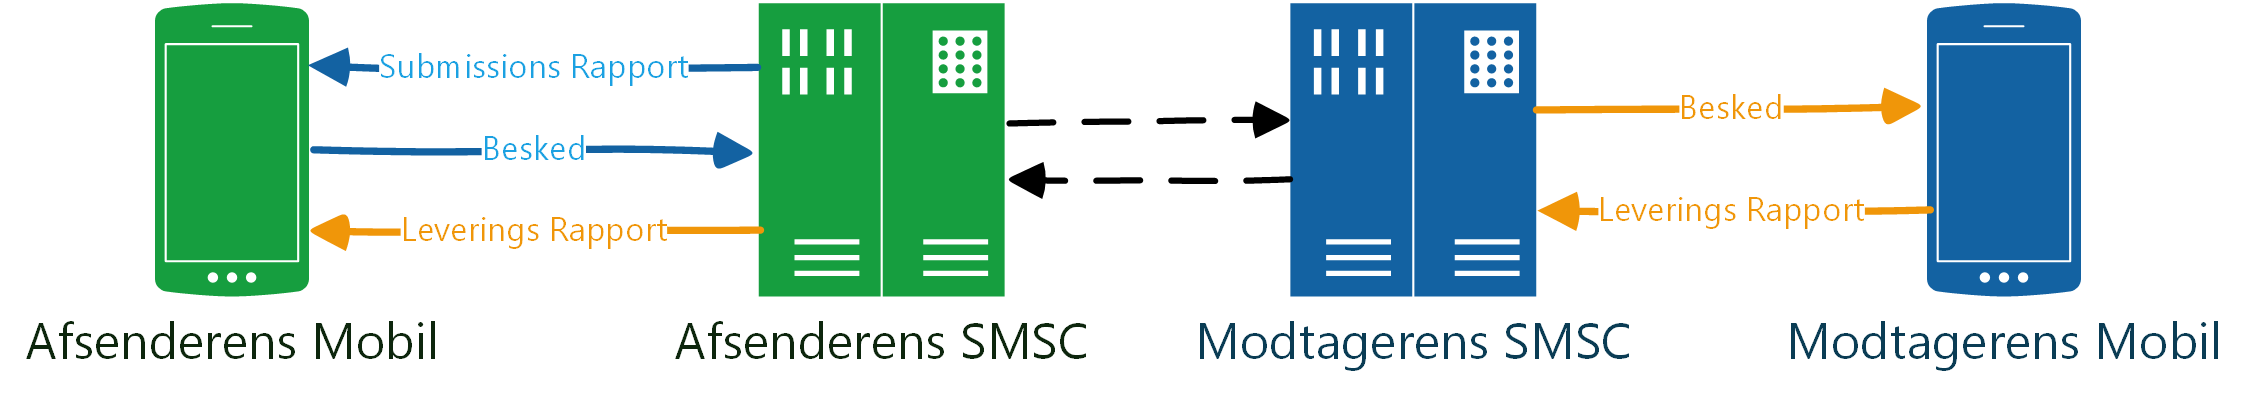
\includegraphics[width=\linewidth]{Billeder/Mobil.png}
\caption {Kommunikationen ved transmission af SMS-beskeder.}
\label{smsTransm}
\end{figure}

Signalerings systemerne i MAP er efter design begrænset til visse størrelser af data. Da man byggede SMS-systemet, talte man tegnene i forskellige beskeder, hvorefter man fandt ud af, at langt de fleste var under 160 tegn. Man mente derfor, at 160 tegn var rigeligt til at rumme de fleste beskeder, hvorved en SMS-beskeds maksimale størrelse blev derfor defineret til 160 tegn. Efter introduktion af udvidede tegnsæt er definitionen præciseret til 1120 bits (160 tegn * 7 bit). \cite{sms_max1} \cite{sms_max2}


Da begrænsningen er defineret i bits, er beskedens maksimale længde afhængig af det anvendte tegnsæt. Det mest almindelige tegnsæt er det grundlæggende 7-bit GSM alfabet. Dette alfabet benytter 7-bits til at symbolisere tegn, hvilket udgør 128 forskellige muligheder. 7-bit GSM alfabetet begrænser derfor en SMS-beskeds længde til 1120/7 bits = 160 tegn. Når der er brug for mere avancerede specialtegn, bruger SMS-systemer UCS-2 tegnsættet. Dette tegnsæt benytter 2 okteter - altså 16 bits - til repræsentation af ét tegn. Ved brug af dette tegnsæt mindskes den maksimale længde derfor ned til 1120/16 = 70 tegn. \cite{sms_pdu}

Enhver SMS-besked indeholder også en header\cite{sms_pdu}, som der er afsat plads til udover de 140 okteter. En SMS-header indeholder typisk data som f.eks. afsenderens telefonnummer, længden af beskeden, benyttet tegnsæt og lignende. Hvis en SMS-besked bliver længere end grænsen, på det benyttede tegnsæt, bliver beskeden delt op i flere beskeder. Når en besked bliver delt op, skrives der information til fletning af beskeden i headeren - og da der ikke er afsat plads til ekstra header information, bliver der brugt 6 okteter af de oprindelige 140 i beskeden. Dette begrænser længden yderligere til 153 ved 7-bit encoding og 67 ved 16-bit encoding. 

	%\clearpage
	
	\section{Tegns�t}
	For at kunne komprimere en besked er det vigtigt at kende til teknologien bag sms’er.

Den teknologi som anvendes i moderne telefoner hedder GSM (Global System for Mobile Communications), som er en 2G standard.# Denne teknologi gør det muligt at benytte sig af sms’er.

For at et computersystem skal have muligheden for at kunne printe tegn til skærmen, er det nødvendig at repræsentere disse tegn med hver sit tal. Disse tal har man bestemt i en standard, som betyder at alle skal benytte de samme tal, for de samme tegn, og derved gøre det lettere for programmørerne af softwaren der benytter disse tegn. Den mest brugte standard indenfor tegnsæt, som dette kaldes, er unicode#

I mobiler der gør brug af GSM, kan der til sms’er, benyttes et tegnsæt kaldt GSM 03.38. Dette tegnsæt kan kodes i en række alfabeter, hvor standard alfabetet GSM 7 bit er et krav ved skabelse af mobiltelefoner.

Nedenunder ses et skema af GSM 7 bit alfabetet:
	%\clearpage
	
	\section{Komprimeringsalgoritmer}
	\subsection{Huffman coding}
Komprimeringsalgoritmen "Huffman coding", er udviklet af David A. Huffman. Huffman udviklede algoritmen, mens han var Ph.D studerende på MIT. I 1952 udgav han dokumentet"A Method for the Construction of Minimum-Redundancy Codes"\cite{A_Method_for}. Her beskrev Huffman, hvordan hans komprimerings algoritme fungerede. Hvad han havde udviklet, var en 'lossless' (tabsfri) komprimerings metode, hvilket betyder, at der ikke vil være noget tab af information ved at komprimere. Komprimeringsmetoden er beregnet til binære systemer, og formålet med algoritmen er at få en given datamænde til at benytte et minimalt antal bit. 

For så at kunne få de orginale data tilbage fra den komprimerede form, kræver det selvfølgelig, at man har en form for ordbog, der beskriver hvilke tegn, der hører sammen med hvilke bits.

For at Huffman coding effektivt kan fungere, skal algoritmen have adgang til hele datamængden, for at kunne analysere hyppigheden af forskellige tegn. Dette betyder at algoritmen skal løbe i gennem datamængden to gange. Første gang, for at indsamle statistik, og anden gang for så at foretage den reelle komprimering. En eksempel på en algoritme der ikke har den ulempe er komprimeringsmetoden "Lempel-Ziv-Welch".


\subsubsection{Generering af Huffman træ}
Huffman algoritmen kigger på frekvensen af tegn, og giver så de hyppigste tegn, den korteste binære kode. For at finde frem til de binære koder til hver tegn, laver man et huffman træ. Træet gør, at den binære kode til et tegn, aldrig vil være starten på koden til et andet tegn. Træet laves ved først at tælle hyppigheden af de forskellige tegn brugt i datamængden der skal komprimeres, og derefter tage de to tegn med lavest frekvens, og lave et nyt punkt, med frekvensen af det første og andet tegn lagt sammen. Dette gøres så indtil der kun er et punkt tilbage. Dette punkt er så toppen af træet. For så at finde frem til den binære kode for hvert tegn, starter man i toppen af træet, og tilføjer 0 eller 1, hvis man gå til henholdsvis venstre eller højre.
\\
\\
Hvis vi kigger på sætningen "dette er et eksempel", viser tabel \ref{tab:huffmantable_new} de forskellige tegn brugt i sætningen, sorteret efter hyppighed. Her tager vi så de to tegn med lavest frekvens (fx D og K), og laver et nyt punkt, med frekvensen af det første og andet tegn lagt sammen. Dette nye punkt, sættes så ind i listen, i stedet for de to tegn. Herefter laves der igen et punkt, med de to tegn/punkter med lavest frekvens, og dette gøres til der kun er et punkt tilbage. Det endelige resultat, bliver så Huffman træet, figur \ref{fig:huffmantree}. 



\begin{figure}[hba]
\centering
\begin{tabular}{|c|c|}
\hline
\cellcolor{ForestGreen}\color{white}{\textbf{Tegn}} &
\cellcolor{ForestGreen}\color{white}{\textbf{Frekvens}} \\ 
\hline 
E & 7 \\ 
\hline 
SPACE & 3 \\ 
\hline 
T & 3 \\ 
\hline 
R & 1 \\ 
\hline 
P & 1 \\ 
\hline 
S & 1 \\ 
\hline 
M & 1 \\ 
\hline 
L & 1 \\ 
\hline 
D & 1 \\ 
\hline 
K & 1 \\ 
\hline 
\end{tabular} 
\caption{Frekvens for tegn i sætningen ''dette er et eksempel''}
\label{tab:huffmantable_new}
\end{figure}

\begin{figure}[H]
\centering
%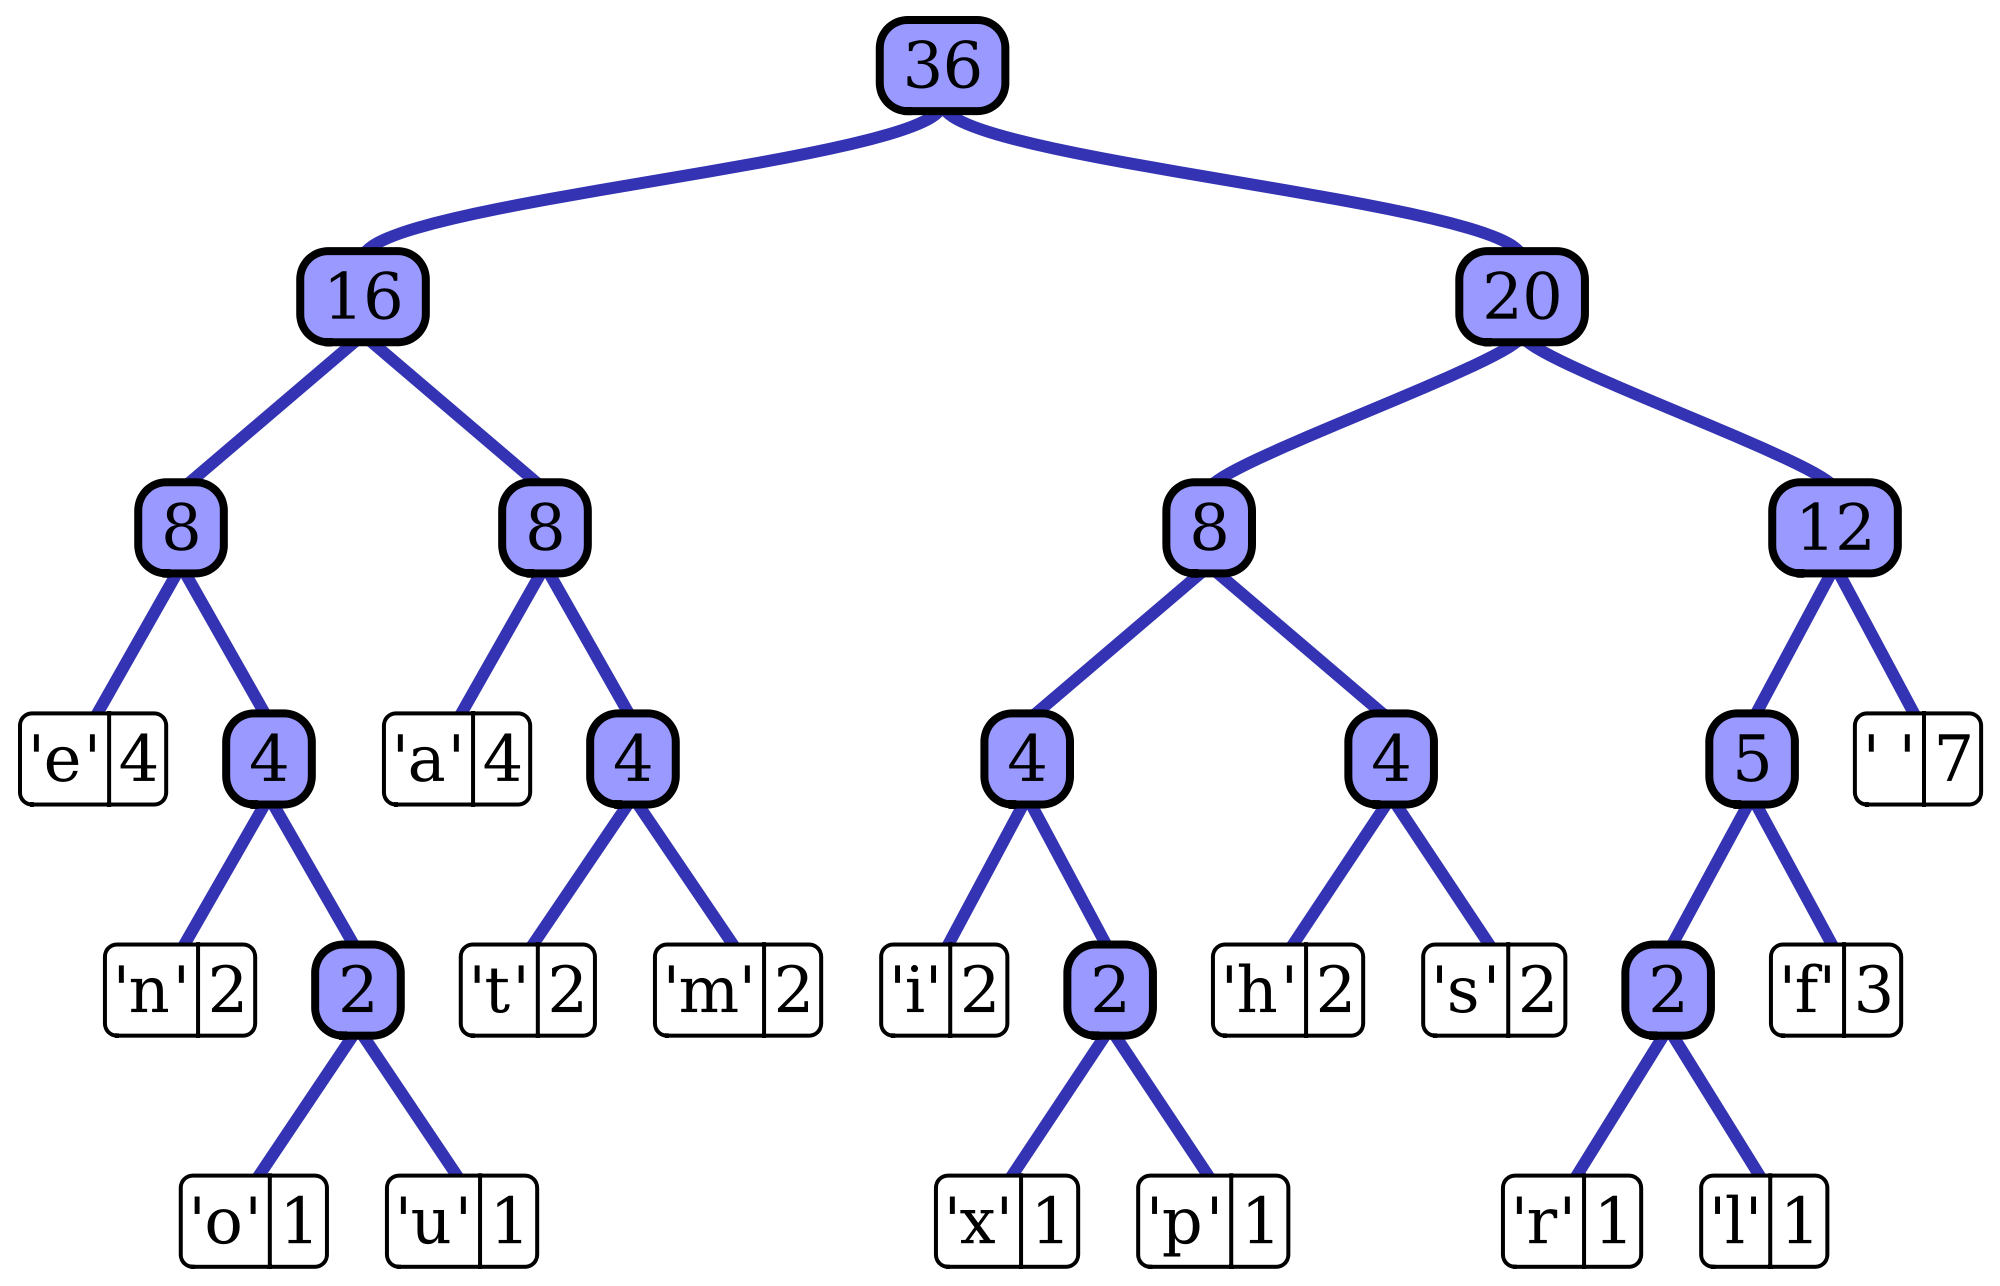
\includegraphics[width=\linewidth]{Billeder/Huffman_tree_2.png}
%

%

%

%
%
%

\enlargethispage{100cm}
% Start of code
% \begin{tikzpicture}[anchor=mid,>=latex',line join=bevel, scale=0.5]
\begin{tikzpicture}[>=latex',line join=bevel, scale=0.8]
  \pgfsetlinewidth{1bp}
%%
\pgfsetcolor{black}
  % Edge: ML -> L
  \draw [->] (271bp,85.689bp) .. controls (271bp,77.317bp) and (271bp,66.99bp)  .. (271bp,47.016bp);
  \definecolor{strokecol}{rgb}{0.0,0.0,0.0};
  \pgfsetstrokecolor{strokecol}
  \draw (274.5bp,64bp) node {1};
  % Edge: 2 -> S
  \draw [->] (127bp,85.689bp) .. controls (127bp,77.317bp) and (127bp,66.99bp)  .. (127bp,47.016bp);
  \draw (130.5bp,64bp) node {1};
  % Edge: 20 -> E
  \draw [->] (115.2bp,388.3bp) .. controls (112.76bp,381.27bp) and (109.84bp,372.85bp)  .. (103.66bp,355.07bp);
  \draw (116.5bp,372bp) node {0};
  % Edge: DK -> K
  \draw [->] (356.54bp,88.329bp) .. controls (365.3bp,78.844bp) and (377bp,66.163bp)  .. (394.43bp,47.282bp);
  \draw (388.5bp,64bp) node {1};
  % Edge: DK -> D
  \draw [->] (343bp,85.689bp) .. controls (343bp,77.317bp) and (343bp,66.99bp)  .. (343bp,47.016bp);
  \draw (346.5bp,64bp) node {0};
  % Edge: 2 -> P
  \draw [->] (113.46bp,88.329bp) .. controls (104.7bp,78.844bp) and (92.997bp,66.163bp)  .. (75.568bp,47.282bp);
  \draw (101.5bp,64bp) node {0};
  % Edge: 7 -> 4
  \draw [->] (213.57bp,242.43bp) .. controls (223.82bp,232.18bp) and (237.71bp,218.29bp)  .. (256.45bp,199.55bp);
  \draw (242.5bp,224bp) node {1};
  % Edge: 13 -> 6
  \draw [->] (158.9bp,315.02bp) .. controls (153.73bp,305.95bp) and (147.15bp,294.39bp)  .. (136.22bp,275.18bp);
  \draw (152.5bp,292bp) node {0};
  % Edge: 4 -> ML
  \draw [->] (271bp,165.69bp) .. controls (271bp,155.89bp) and (271bp,143.42bp)  .. (271bp,122.26bp);
  \draw (274.5bp,144bp) node {0};
  % Edge: 13 -> 7
  \draw [->] (175.19bp,314.3bp) .. controls (178.95bp,305.58bp) and (183.63bp,294.71bp)  .. (191.85bp,275.61bp);
  \draw (191.5bp,292bp) node {1};
  % Edge: 3 -> R
  \draw [->] (113.46bp,168.33bp) .. controls (104.7bp,158.84bp) and (92.997bp,146.16bp)  .. (75.568bp,127.28bp);
  \draw (101.5bp,144bp) node {0};
  % Edge: 6 -> 3
  \draw [->] (127bp,239.94bp) .. controls (127bp,231.81bp) and (127bp,221.88bp)  .. (127bp,202.44bp);
  \draw (130.5bp,224bp) node {0};
  % Edge: ML -> M
  \draw [->] (257.46bp,88.329bp) .. controls (248.7bp,78.844bp) and (237bp,66.163bp)  .. (219.57bp,47.282bp);
  \draw (244.5bp,64bp) node {0};
  % Edge: 20 -> 13
  \draw [->] (131.43bp,389.02bp) .. controls (137.45bp,379.79bp) and (145.16bp,367.99bp)  .. (157.6bp,348.93bp);
  \draw (150.5bp,372bp) node {1};
  % Edge: 3 -> 2
  \draw [->] (127bp,165.69bp) .. controls (127bp,155.89bp) and (127bp,143.42bp)  .. (127bp,122.26bp);
  \draw (130.5bp,144bp) node {1};
  % Edge: 6 -> SPACE
  \draw [->] (110.82bp,243.46bp) .. controls (100.85bp,235.1bp) and (87.659bp,224.06bp)  .. (67.583bp,207.26bp);
  \draw (100.5bp,224bp) node {1};
  % Edge: 7 -> T
  \draw [->] (199bp,239.94bp) .. controls (199bp,233.11bp) and (199bp,225.02bp)  .. (199bp,207.13bp);
  \draw (202.5bp,224bp) node {0};
  % Edge: 4 -> DK
  \draw [->] (284.54bp,168.33bp) .. controls (295.3bp,156.67bp) and (310.52bp,140.19bp)  .. (329.52bp,119.61bp);
  \draw (316.5bp,144bp) node {1};
  % Node: 2
\begin{scope}
  \definecolor{strokecol}{rgb}{0.0,0.0,0.0};
  \pgfsetstrokecolor{strokecol}
  \draw (127bp,104bp) ellipse (27bp and 18bp);
  \draw (127bp,104bp) node {2};
\end{scope}
  % Node: 13
\begin{scope}
  \definecolor{strokecol}{rgb}{0.0,0.0,0.0};
  \pgfsetstrokecolor{strokecol}
  \draw (168bp,332bp) ellipse (27bp and 18bp);
  \draw (168bp,332bp) node {13};
\end{scope}
  % Node: E
\begin{scope}
  \definecolor{strokecol}{rgb}{0.0,0.0,0.0};
  \pgfsetstrokecolor{strokecol}
  \draw (69bp,309bp) -- (69bp,355bp) -- (123bp,355bp) -- (123bp,309bp) -- cycle;
  \draw (97bp,332bp) -- (97bp,355bp);
  \draw (69bp,332bp) -- (123bp,332bp);
  \draw (83bp,337bp) node {E};
  \draw (110bp,337bp) node {7};
  \draw (96bp,314bp) node {0};
\end{scope}
  % Node: D
\begin{scope}
  \definecolor{strokecol}{rgb}{0.0,0.0,0.0};
  \pgfsetstrokecolor{strokecol}
  \draw (316bp,1bp) -- (316bp,47bp) -- (370bp,47bp) -- (370bp,1bp) -- cycle;
  \draw (344bp,24bp) -- (344bp,47bp);
  \draw (316bp,24bp) -- (370bp,24bp);
  \draw (330bp,29bp) node {D};
  \draw (357bp,29bp) node {1};
  \draw (343bp,6bp) node {11110};
\end{scope}
  % Node: SPACE
\begin{scope}
  \definecolor{strokecol}{rgb}{0.0,0.0,0.0};
  \pgfsetstrokecolor{strokecol}
  \draw (0bp,161bp) -- (0bp,207bp) -- (82bp,207bp) -- (82bp,161bp) -- cycle;
  \draw (59bp,184bp) -- (59bp,207bp);
  \draw (0bp,184bp) -- (82bp,184bp);
  \draw (30bp,189bp) node {SPACE};
  \draw (71bp,189bp) node {3};
  \draw (41bp,166bp) node {101};
\end{scope}
  % Node: ML
\begin{scope}
  \definecolor{strokecol}{rgb}{0.0,0.0,0.0};
  \pgfsetstrokecolor{strokecol}
  \draw (271bp,104bp) ellipse (27bp and 18bp);
  \draw (271bp,104bp) node {2};
\end{scope}
  % Node: K
\begin{scope}
  \definecolor{strokecol}{rgb}{0.0,0.0,0.0};
  \pgfsetstrokecolor{strokecol}
  \draw (388bp,1bp) -- (388bp,47bp) -- (442bp,47bp) -- (442bp,1bp) -- cycle;
  \draw (416bp,24bp) -- (416bp,47bp);
  \draw (388bp,24bp) -- (442bp,24bp);
  \draw (402bp,29bp) node {K};
  \draw (429bp,29bp) node {1};
  \draw (415bp,6bp) node {11111};
\end{scope}
  % Node: M
\begin{scope}
  \definecolor{strokecol}{rgb}{0.0,0.0,0.0};
  \pgfsetstrokecolor{strokecol}
  \draw (172bp,1bp) -- (172bp,47bp) -- (226bp,47bp) -- (226bp,1bp) -- cycle;
  \draw (202bp,24bp) -- (202bp,47bp);
  \draw (172bp,24bp) -- (226bp,24bp);
  \draw (187bp,29bp) node {M};
  \draw (214bp,29bp) node {1};
  \draw (199bp,6bp) node {11100};
\end{scope}
  % Node: L
\begin{scope}
  \definecolor{strokecol}{rgb}{0.0,0.0,0.0};
  \pgfsetstrokecolor{strokecol}
  \draw (244bp,1bp) -- (244bp,47bp) -- (298bp,47bp) -- (298bp,1bp) -- cycle;
  \draw (272bp,24bp) -- (272bp,47bp);
  \draw (244bp,24bp) -- (298bp,24bp);
  \draw (258bp,29bp) node {L};
  \draw (285bp,29bp) node {1};
  \draw (271bp,6bp) node {11101};
\end{scope}
  % Node: 3
\begin{scope}
  \definecolor{strokecol}{rgb}{0.0,0.0,0.0};
  \pgfsetstrokecolor{strokecol}
  \draw (127bp,184bp) ellipse (27bp and 18bp);
  \draw (127bp,184bp) node {3};
\end{scope}
  % Node: P
\begin{scope}
  \definecolor{strokecol}{rgb}{0.0,0.0,0.0};
  \pgfsetstrokecolor{strokecol}
  \draw (28bp,1bp) -- (28bp,47bp) -- (82bp,47bp) -- (82bp,1bp) -- cycle;
  \draw (55bp,24bp) -- (55bp,47bp);
  \draw (28bp,24bp) -- (82bp,24bp);
  \draw (42bp,29bp) node {P};
  \draw (69bp,29bp) node {1};
  \draw (55bp,6bp) node {10010};
\end{scope}
  % Node: S
\begin{scope}
  \definecolor{strokecol}{rgb}{0.0,0.0,0.0};
  \pgfsetstrokecolor{strokecol}
  \draw (100bp,1bp) -- (100bp,47bp) -- (154bp,47bp) -- (154bp,1bp) -- cycle;
  \draw (127bp,24bp) -- (127bp,47bp);
  \draw (100bp,24bp) -- (154bp,24bp);
  \draw (114bp,29bp) node {S};
  \draw (141bp,29bp) node {1};
  \draw (127bp,6bp) node {10011};
\end{scope}
  % Node: R
\begin{scope}
  \definecolor{strokecol}{rgb}{0.0,0.0,0.0};
  \pgfsetstrokecolor{strokecol}
  \draw (28bp,81bp) -- (28bp,127bp) -- (82bp,127bp) -- (82bp,81bp) -- cycle;
  \draw (56bp,104bp) -- (56bp,127bp);
  \draw (28bp,104bp) -- (82bp,104bp);
  \draw (42bp,109bp) node {R};
  \draw (69bp,109bp) node {1};
  \draw (55bp,86bp) node {1000};
\end{scope}
  % Node: T
\begin{scope}
  \definecolor{strokecol}{rgb}{0.0,0.0,0.0};
  \pgfsetstrokecolor{strokecol}
  \draw (172bp,161bp) -- (172bp,207bp) -- (226bp,207bp) -- (226bp,161bp) -- cycle;
  \draw (200bp,184bp) -- (200bp,207bp);
  \draw (172bp,184bp) -- (226bp,184bp);
  \draw (186bp,189bp) node {T};
  \draw (213bp,189bp) node {3};
  \draw (199bp,166bp) node {110};
\end{scope}
  % Node: 7
\begin{scope}
  \definecolor{strokecol}{rgb}{0.0,0.0,0.0};
  \pgfsetstrokecolor{strokecol}
  \draw (199bp,258bp) ellipse (27bp and 18bp);
  \draw (199bp,258bp) node {7};
\end{scope}
  % Node: 6
\begin{scope}
  \definecolor{strokecol}{rgb}{0.0,0.0,0.0};
  \pgfsetstrokecolor{strokecol}
  \draw (127bp,258bp) ellipse (27bp and 18bp);
  \draw (127bp,258bp) node {6};
\end{scope}
  % Node: 20
\begin{scope}
  \definecolor{strokecol}{rgb}{0.0,0.0,0.0};
  \pgfsetstrokecolor{strokecol}
  \draw (121bp,406bp) ellipse (27bp and 18bp);
  \draw (121bp,406bp) node {20};
\end{scope}
  % Node: 4
\begin{scope}
  \definecolor{strokecol}{rgb}{0.0,0.0,0.0};
  \pgfsetstrokecolor{strokecol}
  \draw (271bp,184bp) ellipse (27bp and 18bp);
  \draw (271bp,184bp) node {4};
\end{scope}
  % Node: DK
\begin{scope}
  \definecolor{strokecol}{rgb}{0.0,0.0,0.0};
  \pgfsetstrokecolor{strokecol}
  \draw (343bp,104bp) ellipse (27bp and 18bp);
  \draw (343bp,104bp) node {2};
\end{scope}
%
\end{tikzpicture}
% End of code

%



\caption{Huffman træ for sætningen ''dette er et eksempel''}
\label{fig:huffmantree}
\end{figure}


\subsection{Lempel-Ziv-Welch}
Lempel-Ziv-Welch
	%\clearpage
	
	\section{Problemdokumentation}
	N�r det kommer til SMS beskeder, s� er der en gr�nse p� hvor mange tegn der kan v�re i en enkelt besked. For det latinske alfabet ligger begr�nsningen p� 160 tegn. Begr�nsningen �ndrer sig fra tegns�t til tegns�t. For eksempel har det kinesiske alfabet en tegnbegr�nsning p� 70 tegn\cite{Pro_1}. Normalt vil en besked som fylder mere end sin tegnbegr�nsning blive delt op i to separate beskeder, hvis afsenderen af beskeden ikke selv g�r det, hvilket kommer til at betyde dobbelt SMS takst. Med denne begr�nsning i tankerne kommer sp�rgsm�let: Hvor betydeligt er dette problem, og er det overhovedet v�rd at kigge n�rmere p�?
Erhvervs priserne for at sende en SMS inden for Norden og Eurozonen er betydeligt billigere end hvis man sendte til eller fra et Europa land ikke inde under EU, og n�r man sender til eller fra lande udenfor Europa s� bliver det kun dyrere og dyrere. Et internationalt firma som udnytter SMS til intern kommunikation eller andet kan ende med at bruge mange penge p� deres telefonregninger. Tilbage i 2009/2010 begyndte de forskellige telefonselskaber at h�ve prisen p� afsendelse af beskeder til udlandet. TDC's pris, for eksempel, gik fra at v�re p� 2,40 kr. til at koste 3,20 kr. per SMS\cite{Pro_2}. Nedenst�ende tabel viser Telenors SMS takst samt minutpris for erhverv ved at sende beskeder til Danmark, men prisen er stadig den sammen den fra Danmark til udlandet\cite{Pro_3}.

%\noindent
\begin{table}[H]
\begin{center}
\begin{tabular}{ | l | r |}
    \hline
    \cellcolor{ForestGreen} &  \cellcolor{ForestGreen}\color{white}{\textbf{Sende/Modtage SMS}}\\[2ex] \hline
    \textbf{Norden} & 0,66 kr./sms \\ \hline
    \textbf{EU} & 0,66 kr./sms \\ \hline
    \textbf{�vrige Europa} & 3,20 kr./sms \\ \hline
    \textbf{Verden 1} & 3,20 kr./sms \\ \hline
    \textbf{Verden 2} & 3,20 kr./sms \\ \hline
    \textbf{Skibe m. MCP-d�kning} & 3,20 kr./sms \\ \hline
\end{tabular} 
\caption{Tabel over SMS-Priser fra Telenor ~\cite{Pro_3}}
\end{center}
\end{table}

Ligeledes er priserne for private hen over landegr�nserne heller ikke noget at prale af. I det private str�kker priserne sig fra 3's pris pr. SMS p� 2,50 kr\cite{Pro_4} til Telia's pris pr. SMS p� 4,00 kr\cite{Pro_5}. Uanset om man er privat eller erhvervsdrivende s� vil man gerne v�re sparsomme med antallet af beskeder man sender over landegr�nserne, og derudfra g�re god brug af sine 160 tegn s�dan at man undg�r dobbelt SMS takst ved at beskeden bliver delt i to.
Statistikkerne viser at der i 2011 blev sent omkring 12 milliarder SMS?er i Danmark alene, et fald fra forrige �r som l� p� 13 millarder, men det viser at der stadigv�k er h�jst forbrug af SMS beskeder. Derudover s� steg den mobile datatrafik fra 15 milliarder MB i 2010 til 26 milliarder MB i 2011\cite{Pro_6}. En l�sning som komprimere beskeder kunne ogs� hj�lpe til at d�mpe belastningen p� det mobile datatrafik netv�rk.
Derfor vil en eller anden datalogisk l�sning, som g�r det lettere at sende beskede, uden at man skal bekymre som om hvorvidt ens besked har mere end de begr�nsede 160 tegn, v�re aktuelt. S�dan en l�sning kan b�de g�re det mere bekvemt for brugeren at bruge SMS'er, og i det lange l�b sparer brugeren penge.
	%\clearpage
	
	\section{Metodevalg}
	I forbindelse med projektet er der blevet t�nkt over en r�kke metoder, som g�r os i stand til at finde ind til vores problems kerne, og underst�tte problemet i sin helhed.
Ud fra projektforslaget er det blevet fastsat at vores endelige l�sning til problemet skal v�re en prototype af et program. Denne prototype skal v�re skrevet i C, men da problemstillingen omhandler SMS-beskeder, er det  SMS-mediets krav, som vi skal designe vores l�sning efter.


Ud fra vores problem findes der en r�kke interessenter, som p�virkes af denne problemstilling.
P� den f�lgende brainstorm, ses hvordan disse interessenter fordeler sig, ud fra det initierende problem, og hvordan de forbindes til hinanden.

\begin{figure}[H]
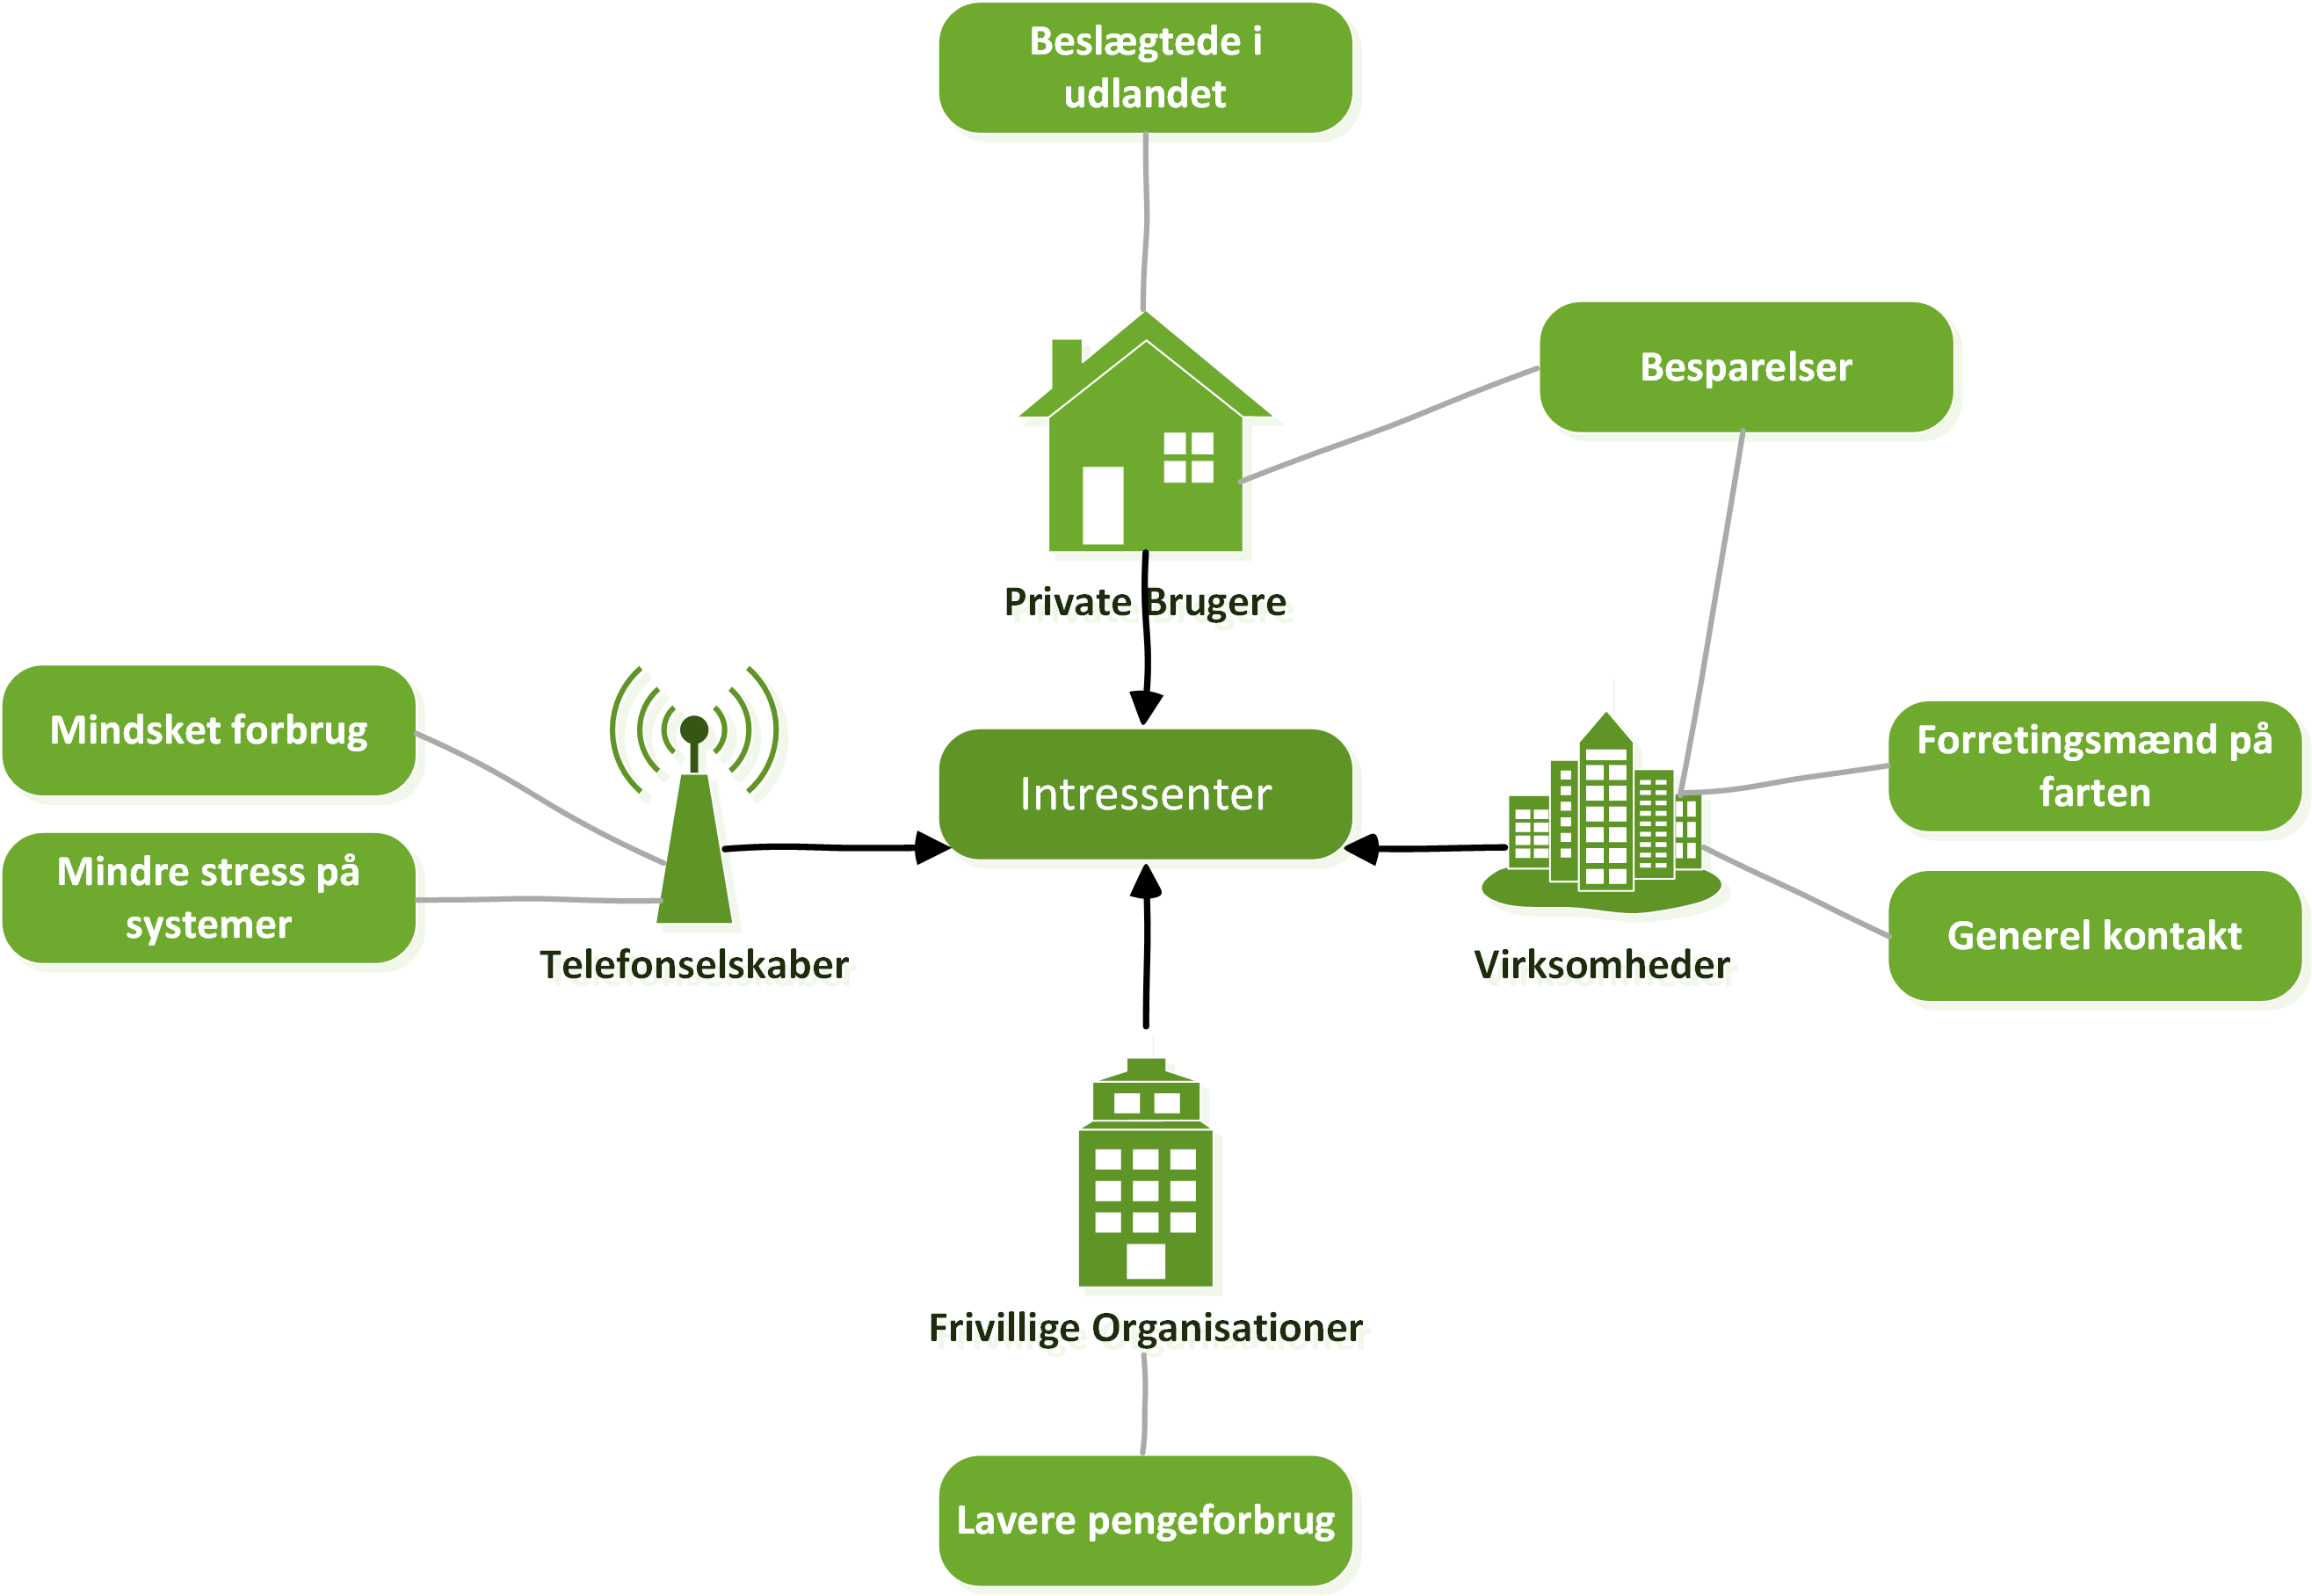
\includegraphics[width=\linewidth]{Billeder/Brainstormting.png}
\caption{Her ses hvordan interessenterne fordeler sig.}
\end{figure}

Denne brainstorm identificerer vores prim�re interessanter, som vil v�re vores hovedm�lgruppe.
Man kan dele interessenterne ind i nogle grupper, henholdsvis: Private personer, Internationale firmaer, Frivillige organisationer og Teleselskaber.
Hver af disse grupper har sin egen grund til at v�re interesseret i vores problemstilling, og derfor kan det ogs� betyde, at der skal forskellige l�sninger til at kunne l�se problemstillingen, for hver forskellig interessant.


Ud fra vores problemstilling findes der en r�kke data som kan v�re anvendelig i forhold til unders�gelsen af de f�rn�vnte interessenter.


Viden om brugen af SMS?er hos de forskellige interessent grupper.
Det er vigtigt at finde ud af hvordan de forskellige interessenter bruger SMS?er som et medie. Med dette menes b�de hvor tit det bruges, men ogs� i hvilken forbindelse og med hvem kommunikationen foreg�r.


Til indsamling af data omkring disse interessanter er det n�dvendigt at komme i direkte kontakt med den m�lgruppe vi har med at g�re. Dette betyder at vi bliver n�dt til at benytte nogle metoder, som g�r det muligt at indsamle eller observere m�lgruppens forbrug af SMS?er.
Til dette vil en sp�rgeskema unders�gelse v�re velegnet, da brugen af SMS?er er data velegnet til kvantitative unders�gelser, da det er et sp�rgsm�l om hvor mange SMS?er der sendes.
	%\clearpage

	\section{Eksisterende L�sninger}
	Der findes flere forskellige former for programmer der allerede helt eller delvist l�ser sms- begr�nsnings problemet. Vi vil i det f�lgende afsnit tage udgangspunkt i to eksisterende programmer.

Det f�rste program hedder SMS ZIP og virker kun til smartphones med Windows som operativsystem. Dette program er af typen ikke tabsfri, da det g�r ind og fjerner alle un�dige mellemrum i teksten, og erstatter f�rste bogstav i f�lgende ord med et stort bogstav, s�ledes at teksten stadig kan l�ses. Ydermere er det programmeret til at kunne identificere bestemte ord og s� erstatte disse med forkortelser. Programmet er indrettet s�ledes at brugeren selv skal v�lge om hver enkelt besked skal komprimeres. Et eksempel p� hvordan programmet vil komprimere en besked:\cite{download-sms} 
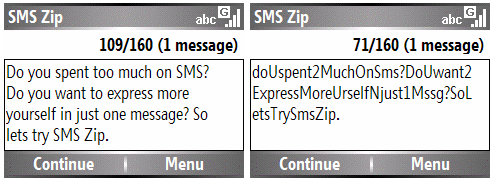
\includegraphics []{Billeder/SMSZIP.png}

Denne konkrete besked bliver alts� kortet ned fra 109- til 71 tegn. En af fordelene ved dette program er at modtageren ikke beh�ver et tilsvarende dekomprimeringsprogram for at kunne l�se beskeden. En anden fordel er at beskeder der ikke overg�r en begr�nsningen, ikke n�dvendigvis bliver komprimeret. Denne l�sning har dog en del flere ulemper end fordele. Den �benlyse ulempe er at beskederne bliver en hel del sv�rere at l�se, og kan v�re en mulig irritation for mange, n�r de l�ser beskeden. En anden klar ulempe er at der bliver brugt en del slang for at g�re ordene kortere, slang s�som tallet ?2? i stedet for ordet ?to?. Dette kan bevirke at budskabet er sv�rere at tage seri�st. Yderligere er det et problem at programmet kun virker til windowsphones og at forkortelserne kun er beregnet til engelsktalende beskeder. Det er derfor, p� baggrund af ovenst�ende, vores vurdering at programmet er en ufuldst�ndig l�sning, og er derfor ikke tilstr�kkelig.\cite{download-sms}

En anden eksisterende l�sning hedder SMS ZIPPER. Det er p� mange punkter et totalt modstridende program i forhold til SMS ZIP. F�rst og fremmest er det forskelligt da dette er et tabsfrit komprimerings program. Programmet virker p� langt de fleste smartphones og er, i mods�tning til SMS ZIP, en l�sning der komprimerer beskeden hos afsenderen og derefter dekomprimerer beskeden igen hos modtageren. Dette kr�ver dog at b�de afsender og modtager har programmet installeret. Programmet starter p� modtagerens telefon liges� snart en komprimeret besked modtages, s� beskeden kan l�ses med det samme uden besv�r for l�seren. Producenten lover helt op til 480 tegn pr. besked, alts� 3 gange s� mange tegn som en almindelig sms. Derudover fungerer programmet til flere sprog, heriblandt dansk, engelsk og tysk.\cite{smszipper} 

Dette program bruger en fleksibel algoritme til at komprimere beskederne. De har designet algoritmen direkte med henblik p� s�kaldte korte beskeder, alts� beskeder omkring de 160 tegn. Endvidere bruger programmet ogs� andre kodnings modeller, som kan v�re beregnet specifikt p� bestemte sprog eller typer af beskeder.

Vi har i ovenst�ende afsnit valgt at tage to vidt forskellige programmer under luppen, for at tegne en kontrast mellem en meget simpel og en mere avanceret l�sning. Vi ser at de hver is�r har deres fordele og ulemper, og disse vil vi tage til overvejelse i vores program.
	%\clearpage

	\section{Afgr�nsning}
	Dette afsnit kommer omkring nogen af de valg, der blev lavet for at indskrænke projektets problemfelt. For det første er der forskellige tjenester og teknologier, som giver muglihed for at sende en kort besked, men med et begrænset antal tegn pr. besked. Eksempelvis er der SMS-beskeder med en begrænsning på 160 tegn når man bruger tegn fra tegnsættet GSM 7-bit\cite{Pro_1} og der er også internettjenester som for eksempel Twitter, som har en tegnbegrænsning på 140 tegn\cite{pro_af1}. Twitters formål har fra starten af, været at give mulighed for at sende korte og smertefrie bidder af information over internettet, og ikke lange blogs og artikler. Denne holdning er folkene bag Twitter meget konsekvente med\cite{pro_af2}. Derudover så er det også gratis at gøre brug af Twitter og derfor er det ikke ligeså væsentligt som SMS, som koster penge. Derfor har vi valgt ikke at arbejde med Twitter. Istedet vil projektet blive begrænset til at handle om SMS-beskeder.

Nu hvor valget om SMS eller Twitter er på plads, så kommer spørgsmålet om hvorvidt der skal arbejdes med smartphones eller almindelige mobiltelefoner. Smartphones har den fordel, at de kan implementere applikation uden alt for meget besvær, hvorimod på almindelige telefoner er det mere besværligt at installere programmer. Statistikkerne viser at flere og flere begynder at få smartphones\cite{pro_af3}. I det sidste kvartal af 2011 blev der solgt over 37 millioner iPhones, Apple's smartphone, i hele verdenen, som er højere end antallet af børn født i den samme periode\cite{pro_af4}. Derudover så bliver der også vist, at brugen af hjemme computere er dallende i det, at adgang til internettet også er tilgængeligt gennem smartphones, som derved gør det muligt for en person at være på internettet hvor man ellers ikke ville have tilgang til en almindelig computer\cite{pro_af3}. Dette kan betyde, at flere personer bruger SMS, fordi de bruger deres mobile enheder mere. Dog kan det også betyde at flere mennesker bruger e-mail i stedet for SMS fordi de alligevel har adgang til internettet. Ud fra dette vil projektet yderligere blive begrænset, til ikke at prøve at implementere programmet på almindelige mobiltelefoner. Derudover så er det også vanskeligt, at implementere en applikation skrevet i C, som er et krav for dette projekt, på en smartphone. Derfor vil løsningen være en prototype, som kan fungere på en computer. 

Når løsningen skal laves, er der brug for en komprimeringsalgoritme. Tidligere er et par komprimeringsalgoritmer blevet gennemgået, for eksempel Huffman eller PPM, som kan bruges til at udvikle løsningen. PPM løsninger har det med at være de bedste til komprimering af tekst. Ligeledes er komprimeringskraften ved Huffman for sig selv også meget kraftig, men er ikke altid optimal. Det er muligt at bygge ovenpå en Huffman komprimeringsalgoritme med PPM. PPM har dog et behov for en del mere RAM i forhold til Huffman, for at kunne komprimere, og er også en langt mere kompliceret løsning at udvikle. Ud fra projektets rammer samt den teoretiske platform som løsningen skulle kunne køre på, en mobiltelefon, så er Huffman løsningen den bedste mulighed. Derfor vil løsningen blive indskrænket til at bruge Huffman som komprimeringsalgoritme.\cite{pro_af5}

Løsningen skal kunne køre uden at forstyrre brugeren af programmet alt for meget. Her gælder blandt andet den tid det tager for programmet at komprimere beskeden, samt hvor meget plads og regnekraft det tager. Det er blandt andet derfor, at det blev besluttet løsningen skulle udvikles ud fra Huffman alene, og ikke lave løsningen med PPM. Ligeledes så skal det heller ikke være nødvendigt for brugeren selv at gøre noget for at komprimere beskeden. Komprimering skal ske automatisk i SMS-processen, uden at brugeren behøver at sætte det igang. Hvis det er nødvendigt med yderlig bruger interaktion, så skal det foregå så brugervenligt som muligt.

Det sidste punkt er hvilke tegnsæt som løsningen skal være i stand til at komprimere og dekomprimere. Skal tegn fra det kyrilliske alfabet eller specialtegn som Æ, Ø, Å og ß være i stand til at blive komprimeret, for eksempel. Det er blevet bestemt, at løsningen skal have implementeret GSM 7-bit tegnsættet, som er standard tegnsættet til SMS-beskeder på mobiltelefoner og smartphone.
	%\clearpage

	\section{Problemformulering}
	Ud fra vores problemanalyse har vi fundet ud af, at der klart er penge at spare, hvis man fra udlandet kan sende én besked i stedet for to. Vi har ligeledes set på eksisterende løsninger som SMS ZIP, for at undgå at lave de fejl, vi mener der er ved de programmer. Derudfra skal vores løsning være mere implementeret, således at brugeren aldrig kommer til at beskæftige sig med den komprimerede besked, så komprimering og dekomprimering sker automatisk. Vi er på baggrund af dette kommet frem til følgende problemformulering:

\begin{itemize}
\item[] \emph{Hvordan kan man spare forbrugeren for dobbelt SMS-takst, ved brug af et komprimeringsprogram? Hvordan kan man undgå at programmet bliver en belastning for brugeren?}
\end{itemize}

Der vil arbejdes frem mod en prototype, der kan komprimere en kort besked, for siden at dekomprimere den på en anden enhed. 	
	%\clearpage
	
	\section{Produktkrav}
	Til dette projekt skal der udarbejdes en løsning i form at et program, som kan komprimere en kort tekstbesked. Komprimeringen vil gøre tekstbeskeden mindre, det vil sige beskeden fylder færre bytes, og skulle gerne både gøre det hurtigere at sende beskeden, fordi den er mindre, men også gøre det muligt at sende en besked over en bestemt tegn begrænsning, som f. eks. de begrænsede 160 tegn ved brug af det latinske alfabet i en SMS. Beskeden skal derefter dekomprimeres hos modtageren, og derefter vise beskeden, som den så ud før den blev komprimeret. Denne proces skal ske, uden brugeren selv tager en direkte del i processen.

\begin {itemize}
\item Funktionelle Krav
\subitem Skal både være i stand til at komprimere og dekomprimere automatisk.
\subitem Programmet skal være i stand til at skelne mellem hvorvidt den pågældende besked skal komprimeres eller dekomprimeres.
\subitem Det er ikke forventet, at prototypen skal kunne køre på en mobil enhed som f. eks. en smartphone, men det er forventet at programmet kan bruges på en computer.

\item Ikke Funktionelle Krav
\subitem Produktet skal afleveres sammen med den tilhørende rapport, og har en fælles deadline den 19 december 2012.
\subitem Programmet skal skrives i programmeringssproget C.

\item Løsningsmål
\subitem Brugeren skal kunne gøre brug af programmet uden selv at tage direkte del i komprimerings-processen.
\subitem Programmet skal køre lokalt, og ligeledes skal komprimeringen og dekomprimeringen også ske lokalt.
\subitem Programmet skal implementeres og være brugbart.
\end{itemize}

	%\clearpage
	
%\chapter{Teori om komprimering?}



\chapter{L�sning}



\chapter{Konklusion}



\begin{thebibliography}{99} %Max
 \bibitem{A_Method_for} D.A. Huffman, {\it Proceedings of the I.R.E.}, September 1952.




%Eksempel:
%\bibitem{DandJ} Dow, W. \& Jones, E.A., {\it Wall Street Journal}, March 29, 1929.

%Eksempel2:
%\bibitem{Simpson} H. Simpson, \emph{Proof of the Riemann
%Hypothesis},  preprint (2003), available at 
%\url{http://www.math.drofnats.edu/riemann.ps}.
\end{thebibliography}

\chapter*{Bilag}
\end{document}